\chapter{Research Methodology}
\label{ch:research-methodology}

\section{Research Model}
\label{sec:research-model}
	\begin{figure}[h]
		\centering
		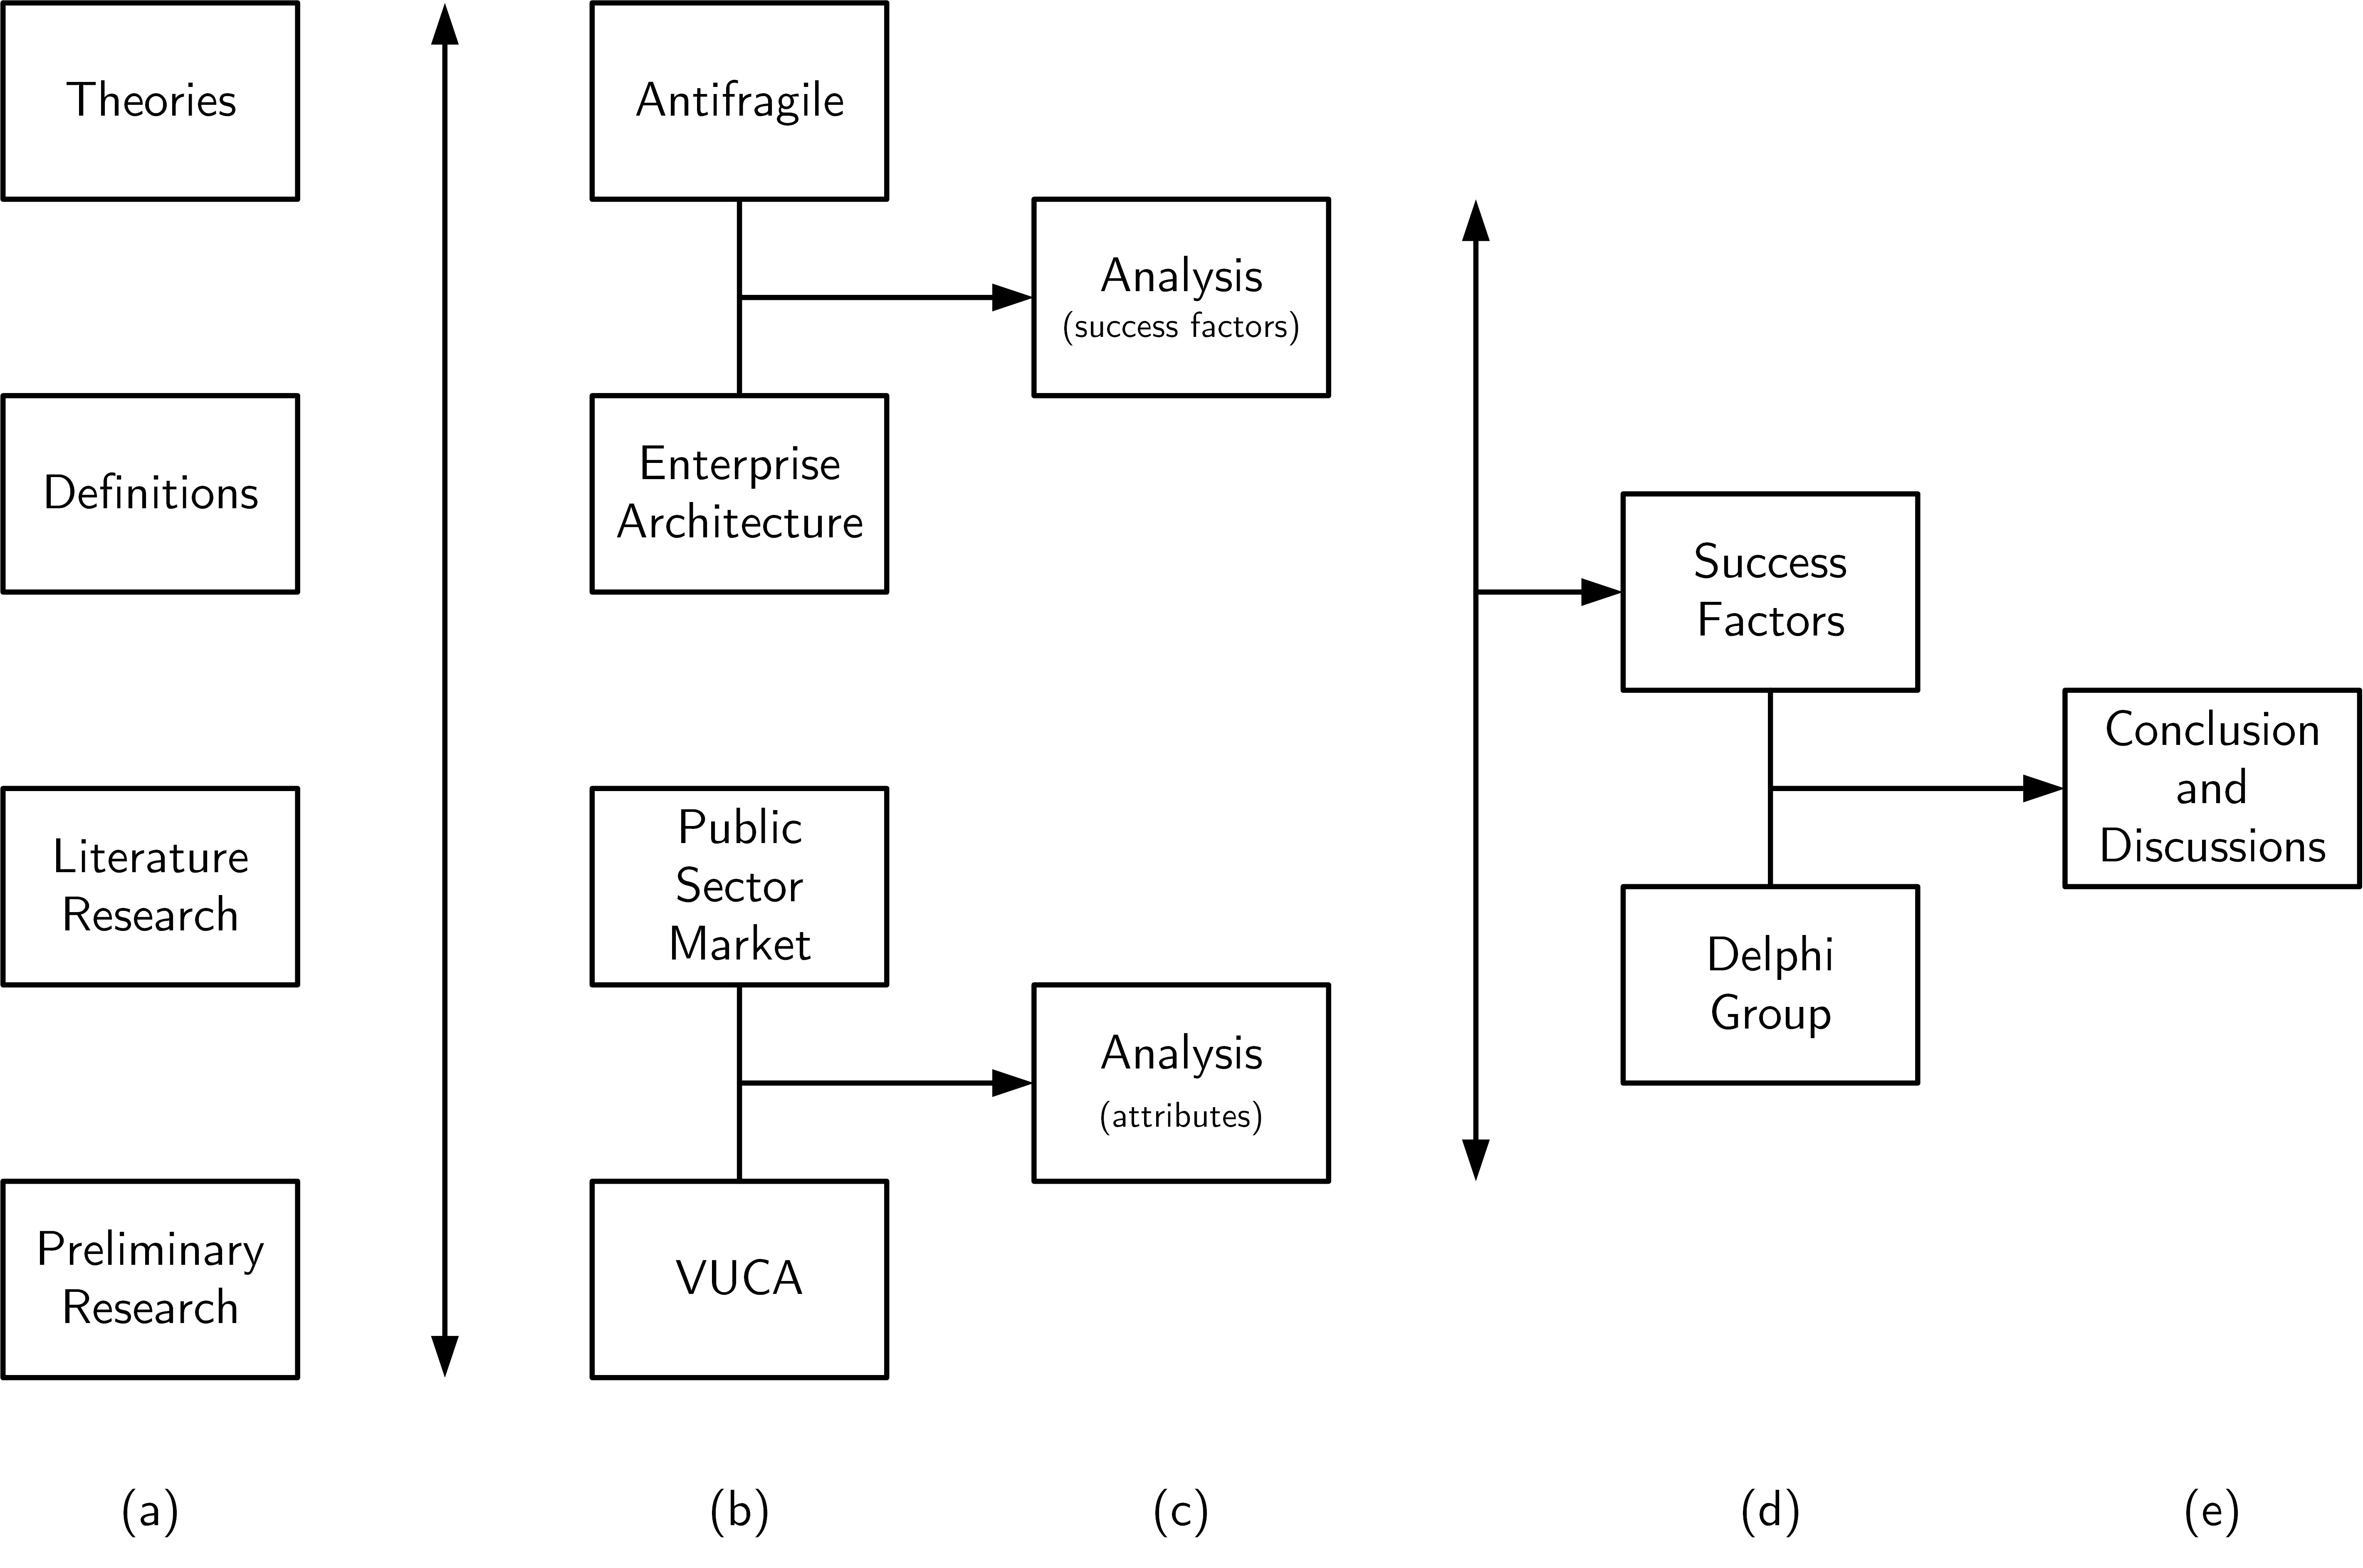
\includegraphics[width=12cm]{images/research-model.png}
		\caption[Research Model]{Research Model}
		\label{fig:research-model}
	\end{figure}

\section{Delphi Group}
For the Delphi Group participants see appendix~\ref{app:delphigroupparticipants} \\%

What about the sample size? Normally Delphi is about 100+. What about this research. How large should the sample size be for a qualitative result?

\section{Quality of the Research (old example text)}
\label{sec:quality-of-the-research}
The research was qualitative. The information is based on qualitative information gathered by the researcher
from employees of the organisation. However, with the research approach and transparency, the research can
be validated, can be repeated, so it is reliable and reducible. With the use of managerial models and methods
like Lean, Value Stream Mapping with supporting tools like NEN-ISO/IEC 25011 and ServQual got a nonbiased
result.
\begin{itemize}
	\item{\textbf{The validity} of the research is dependent on the right use of the right models and the right methods. The researcher conducted research on which models, frameworks and tools to use. The results and the rationales around the choice of theories, models, frameworks and tools are stated in chapter 4. The sources used for determining the theories, models, frameworks and tools are from scientific and expert sources.}
	\item{\textbf{The reliability} is about the influence of possible errors. For the research, the researcher used methods like triangulation, and sources from scientific reports and expert literature. The number of interviews was too small for the right statistical outcome. To enlarge the reliability of the interviews, the researcher used the same framework of themes for his semi-structured interviews. The transcriptions are placed in the appendixes for transparency. The information gathered with the interviewees is compared with the other interviewees.}
	\item{\textbf{The repeatability} is about getting the same results when the research is conducted again. The researcher uses his research design and research approach, as stated. All the steps taken are put into the research design. If this research design is followed, the same results should follow.}
	\item{\textbf{The reducibility} is about the outcome of the research can be deducted step by step. By using the research model, and the structure of the thesis, every step is reducible.}
\end{itemize}

\begin{itemize}
	\item{Think about Replication}
	\item{Recker types}
	\item{OpenScience}
	\item{Howto falsify?}
	\item{Rigourness}
\end{itemize}

Open Science
Open Access
For Replication and transparency.


\parencite[p. 16]{Recker2013}\\
Replicability\\
Falsification\\
Independence\\
Precision\\

The research is using the FAIR Principles\footnote{\url{https://www.go-fair.org/fair-principles/}}\\
\begin{itemize}
	\item{Findable}
	\item{Accesible}
	\item{Interoperable}
	\item{Reusable}
\end{itemize}

\section{Literature research}
For the literature research two methods are used. The first method is (foward and backward) snowballing already found literature. The second method is the use of scientific (online) libraries. The used libraries are:
\begin{itemize}
	\item{Web of Science}
	\item{Research Gate}
	\item{Google Scholar}
\end{itemize}

\noindent A predefined collection of search strings is used for the search with scientific libraries.

\subsection{Search strings}
The following search strings are used for finding literature with the scientific libraries. Not only the full concept name is used but also the abbreviations (eg. Independent Software Vendor and ISV).\\

	\noindent
	\begin{tabular}{p{0.5\textwidth}p{0.5\textwidth}}
		\textbf{\acrlong{ea}} & \\
		Search String 1	&	Search String 2\\%
		Search String 3	&	Search String 4\\%
	\end{tabular}

\vspace{\baselineskip}

	\noindent
	\begin{tabular}{p{0.5\textwidth}p{0.5\textwidth}}
		\textbf{\Gls{antifragile}} & \\
		antifragile robust agile resilient	&	Search String 2\\%
		Search String 3	&	Search String 4\\%
	\end{tabular}

\vspace{\baselineskip}

	\noindent
	\begin{tabular}{p{0.5\textwidth}p{0.5\textwidth}}
		\textbf{\acrlong{isv}} & \\
		Independent Software Vendor antifragile	& Independent Software vendor resilient\\%
		Independent Software Vendor Public Sector	&	Independent Software Vendor Enterprise Architecture\\%
	\end{tabular}

\vspace{\baselineskip}

	\noindent
	\begin{tabular}{p{0.5\textwidth}p{0.5\textwidth}}
		\textbf{Public Sector} & \\
		Difference public and private sector &	Public Sector antifragile\\%
		Public Sector resilient	&	Search String 4\\%
	\end{tabular}

\vspace{\baselineskip}

	\noindent
	\begin{tabular}{p{0.5\textwidth}p{0.5\textwidth}}
		\textbf{Enterprise Architeture \& Antifragile} & \\
		Search String 1	&	Search String 2\\%
		Search String 3	&	Search String 4\\%
	\end{tabular}

\paragraph{Enterprise Architect \& Antifragility}


\paragraph{Public Sector Market \& Independent Software Vendor}

\subsection{Criteria for admission of literature}
It is essential that the literature must help to develop the knowledge necessary to conduct the research. But before the literature can be used the quality of the literature must be evaluated. For evaluating the literature on the usability for this research the criteria accuracy, authority, objectivity, currency, and coverage is used\footnote{\url{https://libguides.library.cityu.edu.hk/litreview/evaluating-sources/}}.



\section{Used infrastructure and tooling}
For selecting the suitable instruments for the research, the Open Science Framework\footnote{\url{https://www.cos.io/products/osf}} is used. The Open Science Framework consists out of 4 stages in a research project. Those stages are: ''Search and Discover, Design Study, Collect and Analyse, and Publish Reports.'' The Open Science Framework proposes specific infrastructure and tools per stage. The transparency in the used infrastructure and tools increases the quality of the research. It increases the replication factor, findability, accessibility, interoperability, and reusability.
\subsection{Thesis creation}
The student used his corporate laptop (Dell Latitude 7200 2-in-1\footnote{\url{https://www.dell.com/en-us/work/shop/dell-laptops-and-notebooks/latitude-7200-2-in-1-laptop/spd/latitude-12-7200-2-in-1-laptop}}) with Windows 10 Professional installed for creating the thesis. The thesis is created with the markup language \LaTeX\footnote{\url{https://www.latex-project.org/}}. The used typesetting environment is TexLive\footnote{\url{https://www.tug.org/texlive/}} with the document type of ''Report'' from KOMA-Script\footnote{\url{https://ctan.org/pkg/koma-script}}. TexStudio\footnote{\url{https://www.texstudio.org/}} is the used \LaTeX\ Editor. It supports syntax-highlighting, has an integrated viewer, reference checking and numerous wizards. For the creation and administration of references Bib\LaTeX\footnote{\url{https://ctan.org/pkg/biblatex/}} is used with the reference manager JabRef\footnote{\url{https://www.jabref.org/}} with the citation style of APA 7th Edition\footnote{\url{https://apastyle.apa.org/}} and with web browser integration. The files are stored on a personal Dropbox\footnote{\url{https://www.dropbox.com/}} that is used by GitHub Desktop\footnote{\url{https://desktop.github.com/}} to synchronise with a public GitHub repository\footnote{\url{https://github.com/JRBliekendaal/master-thesis}}. GitHub\footnote{\url{https://github.com/}} is used for source control but also for reviewing and discussing the topics with the (Co-)Promotor and the planning of the master thesis project. The thesis source files are copied to an Amazon S3 Blob\footnote{\url{https://aws.amazon.com/s3/}} for backup. The backup rotation is seven versions. Cloudberry Explorer Freeware for Amazon S3\footnote{\url{https://www.msp360.com/explorer/windows/amazon-s3.aspx}} is used for backup. Grammarly\footnote{\url{https://www.grammarly.com}}, with the paid subscription service, checks the thesis for spelling, grammar,  style, and plagiarism. The used goals for Grammarly are audience=knowledgeable, formality=formal, and domain=academic. Microsoft Visio Professional\footnote{\url{https://www.microsoft.com/en-ww/microsoft-365/visio/}} is used to create figures. The GitHub repository contains all the sources.
\subsection{Research administration}
\label{tbresearchadministration}
The research administration, which includes documentation containing privacy-sensitive information, like the name and contact information of the Delphi Group participants, is stored on a non-public GitHub Repository\footnote{\url{https://github.com/JRBliekendaal/master-thesis-administration}}. The private GitHub Repository is also for staging thesis parts that still need to be anonymised. For taking notes Leuchtturm1917\footnote{\url{https://www.leuchtturm1917.us/notebook-classic.html}} Notebooks are used with mechanical pencils of Faber-Castell\footnote{\url{https://www.fabercastell.com/products/tk-fine-vario-l-mechanical-pencil-10mm-135900}} and pens from Sakura\footnote{\url{https://www.sakuraofamerica.com/product/pigma-micron/}} with long-lasting ink.
\subsection{Research execution}
\label{sub:tbresearchexecution}
For the execution of the research, Microsoft Excel\footnote{\url{https://www.microsoft.com/en-us/microsoft-365/excel}} is used for the administration of the literature research. For the administration of the literature research, the following headers are used: ID (for a unique ID per item), search terms used, scope, title, subtitle, author(s), year, type, Bib\LaTeX\ citation key, title relevance, abstract relevance, content relevance, found at, doi/isbn, url, date found, duplicate, date used, use for, and notes. Researchgate\footnote{\url{https://www.researchgate.net/}}, Web of Science\footnote{\url{https://app.webofknowledge.com/}}, and Google Scholar\footnote{\url{https://scholar.google.com/}} are the main sources for searching for literature. PaperPanda\footnote{\url{https://paperpanda.app/}} is used for hard to find literature. The literature administration is, together with the publicly available literature, stored in the repository of the master thesis. For non-public available literature, the administration contains the location where the literature is retrievable. All the literature is added to a bib\LaTeX\ file for future reference. For traceability the entries in the bib\LaTeX\ file contain the Unique ID in the notes field. JabRef is used to sort the references by using subgroups to support the workflow. The subgroups used are: ''evaluate, rejected, and used.'' Only the literature in the subgroup used are transferred to the bibliography file of the thesis. This prevents cluttering. For working as paperless as possible all the literature, where possible, is in pdf or in ebook format. For reading Acrobat Reader DC\footnote{\url{https://get.adobe.com/reader/}} is used for reading the PDF, and an Amazon Kindle Oasis\footnote{\url{https://www.amazon.com/dp/B07L5GJD99}} for eBooks. With the Amazon Kindle the highlight feature is used. This is not stored on GitHub since the highlights are under copyright of the author(s).\par
For the execution of the Delphi Method, Meetingwizard\footnote{\url{https://www.meetingwizard.nl/}} is used for questionnaires and the analysis of the questionnaires. The license for using Meeting Wizard is supplied by the Antwerp Management School.